 \documentclass{article}
 \usepackage{graphicx}
 \graphicspath{{ /Pictures/}}

 \begin{document}
\begin{titlepage}
  \begin{center}
    My \LaTeX\ Homework\\
   CASSIOUS KABWE\\
   18/10/2023
  \end{center}
  
 \end{titlepage}
 
 \section{Introduction}
 Hello! This is my first \LaTeX\ document.\\
 This homework is based on the introduction to \LaTeX\ and to know how we can use \LaTeX\ commands and structures to create a well-formated document.
\LaTeX\ is a \textbf{document processor} used to prepare an article, research paper and technicain document.\cite{Smith,J.(2000).A Sample Book}
 
 \section{Main Content}
 \begin{itemize}
    \item Numpy
    \item Pandas
    \item Matplotlib
 \end{itemize}

 The quadratic formula is given by $x=\frac{-b\pm\sqrt{b^2-4ac}}{2a}$.

\subsection{Section A}
\textit{The table below shows the details of a a student at \textbf{MELZARA collage} studying computer science.
his name is James and he is 54 years of age respectively}
\begin{table}[h]
   \caption{Details of a person.}
    \begin{tabular}{|l|c|r|}
        \hline
        Name&James\\ \hline
        Age&54\\ \hline
    \end{tabular}
 \end{table}

 
 \subsection{Section B}
\textbf{A programming language is a system of notation for writing computer programmes.Most programming languages are text-based formal languages but they might also be graphical. Below are some examples of programming languages.}

 \begin{enumerate}
    \item Python 
    \item Kotlin
    \item \LaTeX\
 \end{enumerate}
\begin{figure}
The picture below shows some commands used in creating a document in LaTeX.
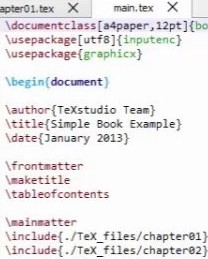
\includegraphics{demo}
\caption{\LaTeX\ page}
\end{figure}
\end{document}

